% Main chapter title
\chapter{Hauptkomponentenanalyse}

% Chapter label
\label{pca}

\section{Motivation}

Die Hauptkomponentenanalyse ist ein weitverbreitetes multivariates statistisches Verfahren zur Dimensionsreduktion. Multivariate Verfahren zielen darauf ab, die in einem Datensatz enthaltene Zahl der Variablen zu verringern, ohne die darin enthaltene Information wesentlich zu reduzieren. Dadurch können umfangreiche Datensätze strukturiert, veranschaulicht und vereinfacht werden. Somit ist das Verfahren Teil der explorativen Statistik, welche Datensätze hinsichtlich ihrer Zusammenhänge analysiert, da nur ein geringes Wissen darüber vorliegt.

Oftmals können sich Gruppierungen / Cluster bilden.

In vielen Bereichen hat die Hauptkomponentenanalyse erfolgreich Anwendung gefunden. Darunter fallen zum Beispiel die Erkennung handgeschriebener Zahlen, welche zum Beispiel zur automatischen Sortierung von Briefen nach Postleitzahl genutzt wird \cite{hastie_elements}, Gesichtserkennung CITE oder in der Genexpressionsanalyse.

Das dahinterstehende mathematische Problem kann auf verschiedene Weisen beschrieben werden. Zunächst wollen wir die Hauptkomponentenanalyse so konstruieren, dass die Idee des minimalen Informationsverlust im Vordergrund steht. Anschließend werden wir das Problem auf eine Singulärwertzerlegung zurückführen, die auch zur effizienten Implementierung genutzt wird. Des Weiteren werden wir die Hauptkomponentenanalyse als Regressionsproblem betrachten und die geometrische Interpretation weiter verdeutlichen. Zu Schluss werden wir einige theoretische Aussagen zeigen.

\section{Konstruktion}

Gegeben sei ein Datensatz mit $n$ samples und $p$ Variablen. Die zentrale Idee der Hauptkomponentenanalyse besteht darin, die $p$ bestehenden Variablen in $r$ neue, unkorrelierte Variablen zu überführen. Um eine Reduktion der Dimension, also $r < p$ zu erreichen, müssen die bestehenden Variablen "zusammengefasst" werden. Idealerweise sollte bei diesem Prozess möglichst wenig Information verloren gehen. Als Maß für den Informationsgehalt der Daten wird hierbei die Varianz verwendet. Das heißt, je größer die Varianz einer Variable, desto mehr Information birgt sie und desto "wichtiger" ist sie. Konkret suchen wir also sukzessive nach einer Linearkombination der bestehenden Variablen. Die entstehenden Vektor zeigen also in die Richtung größter Varianz in unserem Datensatz. Wir nennen sie die Hauptachsen bzw. Hauptrichtungen.

\begin{figure}
\centering
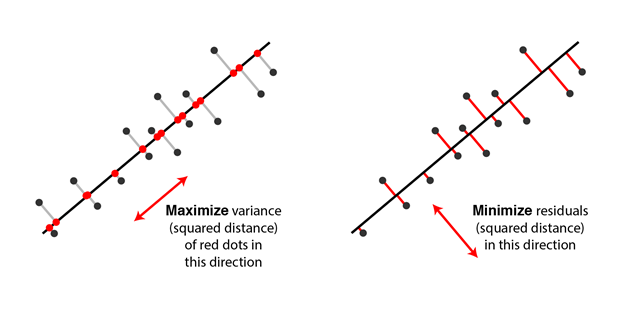
\includegraphics[width = 0.8\textwidth]{figures/pca_projection_explanation.png}
\caption{Die obenstehende Abbildung zeigt die Äquivalenz von Varianzmaximierung und Projektionsdistanzminimierung}
\end{figure}

Abbildung Höhe Gewicht

Um dieses Prinzip zu veranschaulichen, wenden wir uns nun einem simplem Beispiel zu. Gegeben seien die Größe [cm] und das Gewicht [kg] zu 1000 Personen (Daten sind simuliert, keine real-world-data) (siehe dazu Abbildung). In diesem Fall ist also $n = 1000$ und $p = 2$. Bei Betrachtung der Abbildung fällt schnell auf, dass die beiden Variablen positiv korreliert sind, d.h. prinzipiell gibt es die folgende Tendenz: Je größer eine Person, desto schwerer ist sie. Wir können


Konkret konstruieren wir Variablen, die sich aus Linerakombinationen der Alten zusammensetzen. Dabei sollen die neuen Variablen der Wichtigkeit nach sortiert sein. In anderen Worten enthält die erste Variable die meiste Information bzw. die größte Varianz, dann die zweite, usw.
Die eigentliche Dimensionsreduktion findet dann durch Selektierung statt. Je nach Komplexität des Modells und Informationsverlust können so mehr oder weniger ausgewählt werden. Somit haben wir eine kleine, neue Menge an Variablen, die aber trotzdem den Großteil an Informationen / Varianz beinhaltet.

Bevor wir die Hauptkomponentenanalyse auf den Datensatz anwenden können gibt es noch einen wichtigen Bearbeitungsschritt zu beachten. Wenn eine Variable weniger variiert als eine Andere aufgrund der verwendeten Einheit oder Skala (meter oder kilo) kann dies zu ungewollten Ergebnissen führen. Ohne eine Vorbehandlung der Daten hat so zum Beispiel eine Änderung von 1m die gleiche Bedeutung wie eine Änderung von 1kg. Daher werden die Daten oft einem sog. preprocessing unterzogen. Ein oft verwendetes Verfahren ist die Standardisierung (auch z-Transformation genannt). In diesem Schritt werden die Variablen so transfomiert, dass sie "vergleichbarer" werden. Seien dazu $X_i$ die Zufallsvariablen mit Erwartungswert $E[X_i] = \mu$ und Varianz $Var[X_i] = \sigma^2$. So erhält man die zugehörigen standardisierten Zufallsvariablen $Z_i$ durch Zentrierung und anschließender Division durch die Standardabweichung $Z = \frac{X-\mu}{\sigma}$. Somit gilt:
\begin{itemize}
\item $E[Z_i] = 0$ für alle $1 \leq i \leq p$
\item $Var[Z_i] = 1$ für alle $1 \leq i \leq p$
\end{itemize}


Diese Dinge müssen noch irgendwo untergebracht werden im Text:
\begin{itemize}
\item Mathematisch wendet man das Verfahren also nicht auf die Kovarianzmatrix, sondern auf die Korrelationsmatrix an.
\item Anordnung nach absteigender Varianz bzw. Information
\item Hauptkomponente vs Hauptachse
\item Wir gehen von einem vollständigem Datensatz aus bei dem keine Einträge fehlen bzw. korrupt sind. Entsprechende Erweiterungen existieren in cite und cite. 
\item Annahmen: Keine Außreiser, Lineare Verteilung
\item No, PCA is not selecting some characteristics and discarding the others. Instead, it constructs some new characteristics that turn out to summarize our list of wines well. Of course these new characteristics are constructed using the old ones
\item Indeed, imagine that you come up with a property that is the same for most of the wines. This would not be very useful, wouldn't it? Wines are very different, but your new property makes them all look the same! This would certainly be a bad summary. Instead, PCA looks for properties that show as much variation across wines as possible.
\item ortogonale Projectionen
\end{itemize}


\subsection{Problemformulierung als Varianzmaximierung}

Wir wollen nun die Intuition des minimalen Informationsverlust mathematisch formulieren. Gegeben sei dazu eine Matrix $\mat{X} \in \mathbb{R}^{n\times p}$, wobei $n$ die Anzahl der Samples bzw. Beobachtungen und $p$ die Anzahl der Variablen ist. Ohne Beschränkung der Allgemeinheit nehmen wir im Folgenden an, dass die Daten zuvor standardisiert wurden.
Aufgabe der Hauptkomponentenanalyse ist es nun sukzessive die Richtungen größter Varianz zu finden und anschließend die Daten auf die neu konstruierten Variablen zu projizieren. Mathematisch können erhalten wir die erste Hauptachse dann durch:
$$v_1 = \argmax_{\norm{v}_2 = 1} \sum_{i=1}^n(X_iv)^2 = \argmax_{\norm{v}_2 = 1} \norm{Xv}_2^2 = \argmax_{\norm{v}_2 = 1} v^T \mat{K}_{xx} v$$
wobei $\mat{K_{xx}}$ die Kovarianzmatrix ist. Die erste Hauptkomponente, d.h. die Projektion der Daten auf die erste Hauptachse erhält man durch $Z_1 = \sum_{j=1}^{p} v_{1j}X_j$, wobei $v_1 = (v_{11}, \ldots, v_{1p})^T$. Die restlichen Hauptachsen und Komponenten können sukzessive definiert werden.
$$v_{k+1} = \argmax_{\norm{v} = 1} v^T \mat{K}_{xx} v$$ unter der Nebenbedingung, dass $v_{k+1}^Tv_l = 0, \forall 1 \leq l \leq k$. Man sucht also unter den Richtungen, die orthogonal zu allen bisherigen Hauptachsen sind, diejenige, die die Varianz maximiert.
\cite{zou_overview}
CITE JOLLIFE

Wie wir bereits in THEOREM gesehen haben, entsprechen die Eigenvektoren der Kovarianzmatrix genau den Richtungen maximaler Varianz wie oben definiert. Daher können wir anstatt sukzessiver Berechnung einzelner Hauptachsen die Kovarianzmatrix $\mat{K}_{xx}$ diagonalisieren. Da $\mat{K}_{xx}$ symmetrisch ist
$$\mat{K}_{xx} = \mat V \mat L \mat{V}^T$$
wobei $\mat V$ die Matrix der Eigenvektoren ist (Jede Spalte ist ein Eigenvektor) und $\mat{L}$ ist eine Diagonalmatrix mit Eigenwerten $\lambda_i$ in absteigender Reihenfolge. Die Eigenvektoren entsprechen den Hauptachsen und die Projektion der Daten auf die Hauptachsen wird erreicht durch Multiplikation des Datensatz mit den Eigenvektoren $\mat Z = \mat X \mat V$. Die Spalten in $\mat{Z}$ sind also die Hauptkomponenten. Die i-te Beobachtung bezüglich der neuen Variablen sind die Zeilen von $\mat{X}\mat{V}$.



 Wie wir bereits in CITE gesehen haben, entsprechend diese Richtungen genau den Eigenvektoren der Stichprobenkovarianzmatrix. Die Stichprobenkovarianzmatrix ist gegeben durch $\mat{K}_{xx} = \frac{(\mat{X}^T\mat{X})}{n}$. 
 
 If we now perform singular value decomposition of X, we obtain a decomposition
X=USV⊤,
where U is a unitary matrix and S is the diagonal matrix of singular values si. From here one can easily see that
C=VSU⊤USV⊤/(n−1)=VS2n−1V⊤,
meaning that right singular vectors V are principal directions and that singular values are related to the eigenvalues of covariance matrix via λi=s2i/(n−1). Principal components are given by XV=USV⊤V=US

.

To summarize:

    If X=USV⊤

, then columns of V
are principal directions/axes.
Columns of US
are principal components ("scores").
Singular values are related to the eigenvalues of covariance matrix via λi=s2i/(n−1)
. Eigenvalues λi
show variances of the respective PCs.
Standardized scores are given by columns of n−1−−−−−√U
and loadings are given by columns of VS/n−1−−−−−√
. See e.g. here and here for why "loadings" should not be confused with principal directions.
The above is correct only if X
is centered. Only then is covariance matrix equal to X⊤X/(n−1)
.
The above is correct only for X
having samples in rows and variables in columns. If variables are in rows and samples in columns, then U and V
exchange interpretations.
If one wants to perform PCA on a correlation matrix (instead of a covariance matrix), then columns of X
should not only be centered, but standardized as well, i.e. divided by their standard deviations.
To reduce the dimensionality of the data from p
to k<p, select k first columns of U, and k×k upper-left part of S. Their product UkSk is the required n×k matrix containing first k
PCs.
Further multiplying the first k
PCs by the corresponding principal axes V⊤k yields Xk=UkSkV⊤k matrix that has the original n×p size but is of lower rank (of rank k). This matrix Xk provides a reconstruction of the original data from the first k
PCs. It has the lowest possible reconstruction error, see my answer here.
Strictly speaking, U
is of n×n size and V is of p×p size. However, if n>p then the last n−p columns of U are arbitrary (and corresponding rows of S are constant zero); one should therefore use an economy size (or thin) SVD that returns U of n×p size, dropping the useless columns. For large n≫p the matrix U would otherwise be unnecessarily huge. The same applies for an opposite situation of n≪p.

\subsection{Formulierung als Singulärwertzerlegung}
$$ \mat{X} = \mat{U}\mat{D}\mat{V}^T $$
wobei $\mat{D}$ eine Diagonalmatrix mit Elementen $d_1,\ldots,d_p$ in absteigender Reihenfolge, $\mat{U}$ eine $n \times p$ und $\mat{V}$ eine $p \times p$ orthogonale Matrix.
$\mat{U}\mat{V}$ sind die Hauptkomponenten und die Spalten von $\mat{V}$ sind die Eigenvektoren von $\mat{X}$.

\subsection{Formulierung als Regressionsproblem}
$$\hat{\mat{V}_k} = \argmin_{\mat{V}_k} \sum_{i=1}^{n} \norm{x_i - \mat{V}_k \mat{V}_k^Tx_i}^2 + \lambda \sum_{j=1}^{k}\norm{\beta_j}^2$$

subject to $\mat{V}_k^T\mat{V}_k = I_{k \times k}$

\cite{zou_sparsepca}

Man projiziert die Daten auf einen k-dimensionalen linearen Unterraum. Man kann zeigen, dass die Lösung dieses Problem genau die ersten k Hauptachsen sind.

Ausgehend von dieser Formulierung als Regressionsproblem werden wir im nächsten Kapitel die Variante der dünnbesetzten Hauptkomponentenanalyse beschreiben.

\section{Theoretische Aussagen}

\begin{thm}
PCA always gives unique solution.
\end{thm}

\begin{thm}[\cite{vidal}]
Sei $\mat X \in \mathbb{R}^n$ und $\mat A_{p,k} = [\alpha_1, \ldots \alpha_k] $   
\end{thm}

\begin{thm}
PCA inconsistent for p >> n.
\end{thm}

\section{Limitations}

PCA Limitations

Model performance: PCA can lead to a reduction in model performance on datasets with no or low feature correlation or does not meet the assumptions of linearity.

Classification accuracy: Variance based PCA framework does not consider the differentiating characteristics of the classes. Also, the information that distinguishes one class from another might be in the low variance components and may be discarded.

Outliers: PCA is also affected by outliers, and normalization of the data needs to be an essential component of any workflow.

Interpretability: Each principal component is a combination of original features and does not allow for the individual feature importance to be recognized.

